Nick Vosseteig

2014-10-10

brainstorming, helping other teams, and testing.

\begin{tabular}{|p{5cm}|p{5cm}|}
 \hline
 Brainstorming&
We brainstormed methods to repeatedly fire our slingshot and came up with two possible solutions of a winch with a clutch, and a wheel attached to the ball-holder.
 \\
 \hline
helping other teams&
I continued helping the other teams since they are less experienced with programming. David set up the hardware to test simple programs by using the joystick. This week I also set up a few sample programs that people can reference or test out with the hardware to see how the code works. 
 \\
 \hline
 testing&
We tested out the surgical tubing by using a makeshift launcher with 2 chairs and a cup attached to the tube in order to test launching the balls. We determined that it does not need to be pulled down very far to launch the balls as high as we need to, but it takes a substantial amount of force to pull down. If we use less tension, it needs to be pulled down further, but takes less force to do it, but having a much shorter, higher tension launcher could increase reliability and make the mechanism easier to work with.
 \\
 \hline
\end{tabular}

\section*{Helping other teams}
Helping the other teams with programming is something that I've been working on alot and this week I came up with some short sample code to show them:

\lstinputlisting[style = RobotC]{ServoTest.c}

It's very simple code, but it helps them to understand how to set up their code and allows them to understand this simple code on how to use a servo motor with the joystick controller.

\section*{Testing}
We tested out the surgical tubing, but the problem is whether we should use a lot of tension or a little tension. There are pros and cons to both sides: Having less tension means that the tubing needs to be pulled further down, but it would be less hard on the motor doing it, having more tension puts more pressure on the motor, but allows for a more reliable, and more compact slingshot.

\begin{center}
% 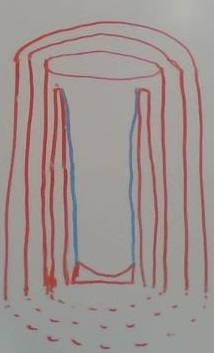
\includegraphics[width=10cm]{./Entries/Images/launcher.png}
 %launcher.png: 740x709 pixel, 90dpi, 20.89x20.01 cm, bb=0 0 592 567
\end{center}
